\subsection{Measurement Data}\label{sec:cloud:virtualized_network_functions:measurement_data}

In order to evaluate our models introduced in \refsec{sec:cloud:virtualized_network_functions:model}, we use data gathered from a nation-wide mobile operator.
This allows for precise core network evaluations and the creation statistical fits for the observed processes.
In this section we first describe the dataset used for the evaluation and afterwards, we derive the random variables required for our models.

\subsubsection*{Dataset Description}\label{sec:cloud:virtualized_network_functions:measurement_data:description}

\label{sec:dataset_description}

All data was collected by the \gls{METAWIN} monitoring system~\cite{Ricciato2006} with measurement probes located at the Gn interface within the core network, enabling broad access to signalling.
For this investigation we employ \gls{GTP} protocol data gathered by \gls{METAWIN}.
This data includes the \gls{RAT} identifier as well as the terminal types of the mobile clients, by use of the \gls{TAC} part of the \gls{IMEI}.
To meet privacy requirements, \gls{METAWIN} anonymises all captured data.
The application-level payload is removed and all user identifiers are hashed with one-way functions before data storage.
Individual \glspl{UE} in our dataset can be differentiated by the hashed \gls{MS-ID}, but not traced back to the actual user.

The used dataset is a week-long trace from the third week of April 2011.
It consists of \(2.2\) billion aggregated flows for user traffic and \(410\) million \gls{GTP} Tunnel Management transactions.
It was tapped at one of the \glspl{GGSN} of the operator and contains about half of the total traffic volume handled by the operator in this period.

\subsubsection*{Statistical Evaluation}\label{sec:cloud:virtualized_network_functions:measurement_data:evaluation}

Using this dataset, we can obtain the distributions required for the models introduced in \refsec{sec:cloud:virtualized_network_functions:model}.
First, we study the tunnel inter-arrival time in \reffig{fig:cloud:virtualized_network_functions:measurement_data:evaluation:tunnel_iat}.

\begin{figure}
  \centering
  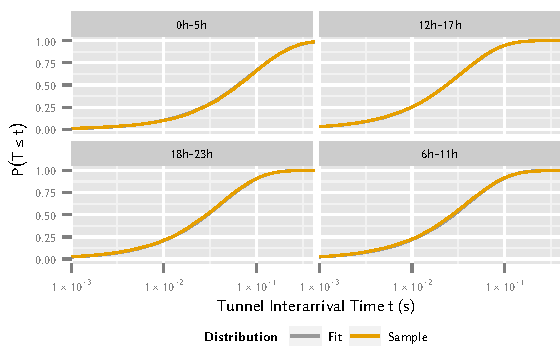
\includegraphics{cloud/virtualized_network_functions/measurement_data/figures/tunnel_iat}
  \caption{Empirical and exponentially fitted \headershortacrpl{CDF} of the tunnel inter-arrival duration by time of day. \headershortacrpl{CDF} are overlapping as the coefficient of determination is close to \(1\).}
  \label{fig:cloud:virtualized_network_functions:measurement_data:evaluation:tunnel_iat}
\end{figure}

The arrival of new tunnel requests can be used as a measure for the load a \gls{GGSN} experiences, as every incoming tunnel carries several signalling interactions, processing and state with it.
Typically, a device will only hold one tunnel at a time, but this tunnel can be initiated and shut down in rapid succession, causing the aforementioned issues in the radio network.
The arrivals also show a strong diurnal effect, closely resembling patterns present in the actual user traffic:
We observe a decline of arrivals, i.e. longer inter-arrivals, late in the night and during the early morning hours with a peak rate in the afternoon and early evening.
To represent this time-of-day dependence in the model, the measurement was split into the four time slots displayed in the figure.
Each slot was then fitted with an exponential distribution by way of moment matching.
This results in the cumulative negative exponential distribution function \(F(x) = 1- e^{-\lambda x}, x \geq 0\) with \(\lambda\) given in \reftab{tab:cloud:virtualized_network_functions:measurement_data:evaluation:iat_fits} for the four time slots.
The fitted functions match the empirical data, with some deviation present at the left tail but overall with a positive correlation coefficient approaching \(1\).

\begin{table}
  \centering
  \caption{Parameters for the exponentially distributed inter-arrival times and corresponding Pearson correlation coefficients.}
  \label{tab:cloud:virtualized_network_functions:measurement_data:evaluation:iat_fits}  
  \begin{tabular}{lcc}
  \toprule
  Time of day & \(\lambda\) & \(R_{arr}\)\\
  \midrule
  0h-5h & $10.67$ & $0.99$\\
  6h-11h & $24.53$ & $0.99$\\
  12h-17h & $29.25$ & $0.99$\\
  18h-23h & $23.49$ & $0.98$\\
   \bottomrule
  \end{tabular}
\end{table}

The second important tunnel property is the duration of the \gls{PDP} Context state accompanying a \gls{GTP} tunnel held at the \gls{GGSN}.
\reffig{fig:cloud:virtualized_network_functions:measurement_data:evaluation:tunnel_duration} shows the tunnel durations split up for the time of day, as there is once again a slight diurnal effect present, albeit with shifted peaks.
Longer tunnels tend to occur at night, shorter tunnels during midday.
Further properties of the tunnel duration, especially the correlation with device types and operating systems, are investigated in detail in~\cite{Metzger2014}.

\begin{figure}
  \centering
  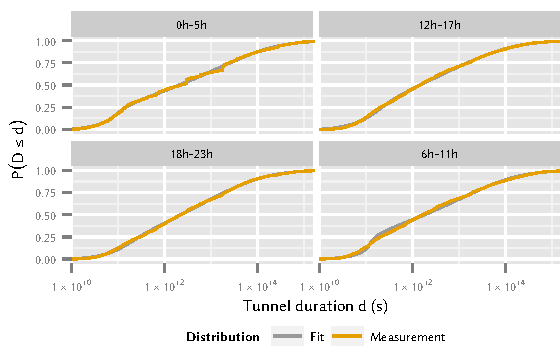
\includegraphics{cloud/virtualized_network_functions/measurement_data/figures/tunnel_duration}
  \caption{Empirical and fitted \headershortacrpl{CDF} of the tunnel duration by time of day with fitted rational functions.}
  \label{fig:cloud:virtualized_network_functions:measurement_data:evaluation:tunnel_duration}
\end{figure}

\begin{table}
  \centering
  \caption{Inverse functions fitted to the empirical duration distribution and correlation coefficients of the fit.}
  \label{tab:cloud:virtualized_network_functions:measurement_data:evaluation:duration_fits}  
  \begin{tabular}{lcc}
  \toprule
  Time of day & Inverse fitted duration function & \(R_{dur}\)\\
  \midrule
  0h-5h & $0.91 - 60.61y - 3498.78y^3 - \frac{110.70y + 2289.94y^3}{y - 1.00}$ &  $0.99$ \\
  6h-11h & $1 + 117.48y - 368.64y^2 - \frac{1720.13y^4}{y - 1.00}$ & $0.99$ \\
  12h-17h & $0.95 + 69.49y + \frac{81146.10y^3 + 1.08\times10^6y^5}{805 - 802.01y}$ & $0.99$ \\
  18h-23h & $0.91 + 82.05y - \frac{2936.93y^4}{1.94y - 1.95}$ & $0.99$\\
  \bottomrule
  \end{tabular}
\end{table}

Furthermore, the model requires information on the tunnel durations.
However, none of the basic probability distributions, e.g. exponential, gamma, and weibull distributions, fit the tunnel duration well enough.
One of the reasons for this probably being the correlation of the tunnel duration to a large number of factors, including user behaviour and network-specific timers and procedures, e.g. tunnels are shut down by the network after specific events, introducing artefacts which make it hard to fit any distribution against.
Instead, we fit rational functions to the empirical \gls{CDF} using the Eureqa \cite{Schmidt2009} software.

This allows for a much closer fit while still smoothing out some of the artefacts.
\reftab{tab:cloud:virtualized_network_functions:measurement_data:evaluation:duration_fits} displays these functions fitted to the inverse \gls{CDF}, to be directly used for generating random numbers using the inversion method.
Both the \gls{CDF} in \reffig{fig:cloud:virtualized_network_functions:measurement_data:evaluation:tunnel_duration} as well as the Pearson correlation coefficient confirm the goodness of the fitted functions.
